\documentclass[letterpaper,12pt]{article}
\usepackage{tabularx} % extra features for tabular environment
\usepackage{amsmath}  % improve math presentation
\usepackage{graphicx} % takes care of graphic including machinery

\usepackage[margin=1in,letterpaper]{geometry} % decreases margins
\usepackage{cite} % takes care of citations
\usepackage[final]{hyperref} % adds hyper links inside the generated pdf file
\bibliographystyle{plain}
\hypersetup{
	colorlinks=true,       % false: boxed links; true: colored links
	linkcolor=blue,        % color of internal links
	citecolor=blue,        % color of links to bibliography
	filecolor=magenta,     % color of file links
	urlcolor=blue         
}
\usepackage{blindtext}
%++++++++++++++++++++++++++++++++++++++++


\begin{document}

\title{Report on \textbf{Project: Computer simulations of molecular liquids}}
\author{Zhicheng Zhang}
\date{\today}
\maketitle

\begin{abstract}
In this project, I applied molecular simulation methods to studying the properties of a 2D system of particles. The methods include molecular dynamics (MD) and Metropolis Monte Carlo (MC) simulation. I modeled the system using different model interaction potentials among the particles, including Lennard-Jones (LJ) potential, model atomic potential and model colloidal potential, all pairwise and with a cut-off distance $r_c$. With carefully chosen initial conditions and boundary conditions, I was able to realize equilibrium states, calculate average total energies and deviations, calculate the radial distributions functions, evaluate the pressure, etc. \textbf{Special notes:} 
\end{abstract}


\section{Introduction}

This is the final project of the course Introduction to Computational Physics. The project is aimed at testing our ability to implement the algorithms we learned in class through programming. The 

\section{Background}

Give a brief summary of the physical theory, include any equations necessary, and cite any references you want to include. Here is how you insert an equation. According to
references~\cite{melissinos, Cyr, Wiki} the dependence of interest is given
by
\begin{gather*}
   \mathcal{L} =  \frac{1}{2} m \ell^2 ( \dot{\theta}+\dot{\phi}_0)^2 - m g_e(t) \ell \cos(\theta)\\
   \\
   m\ell^2 (\ddot{\theta} + \ddot{\phi}_0) = mg_e\ell\sin(\theta)\\
\end{gather*}
\begin{equation}
   \ddot{\phi}(t) = -\frac{g_e(t)}{\ell} \sin\left(\phi(t)-\phi_0(t)\right)
   \label{Eq:equation1} %the label lets you refer to the equation later
\end{equation}

\begin{figure}[!h]
    \centering
    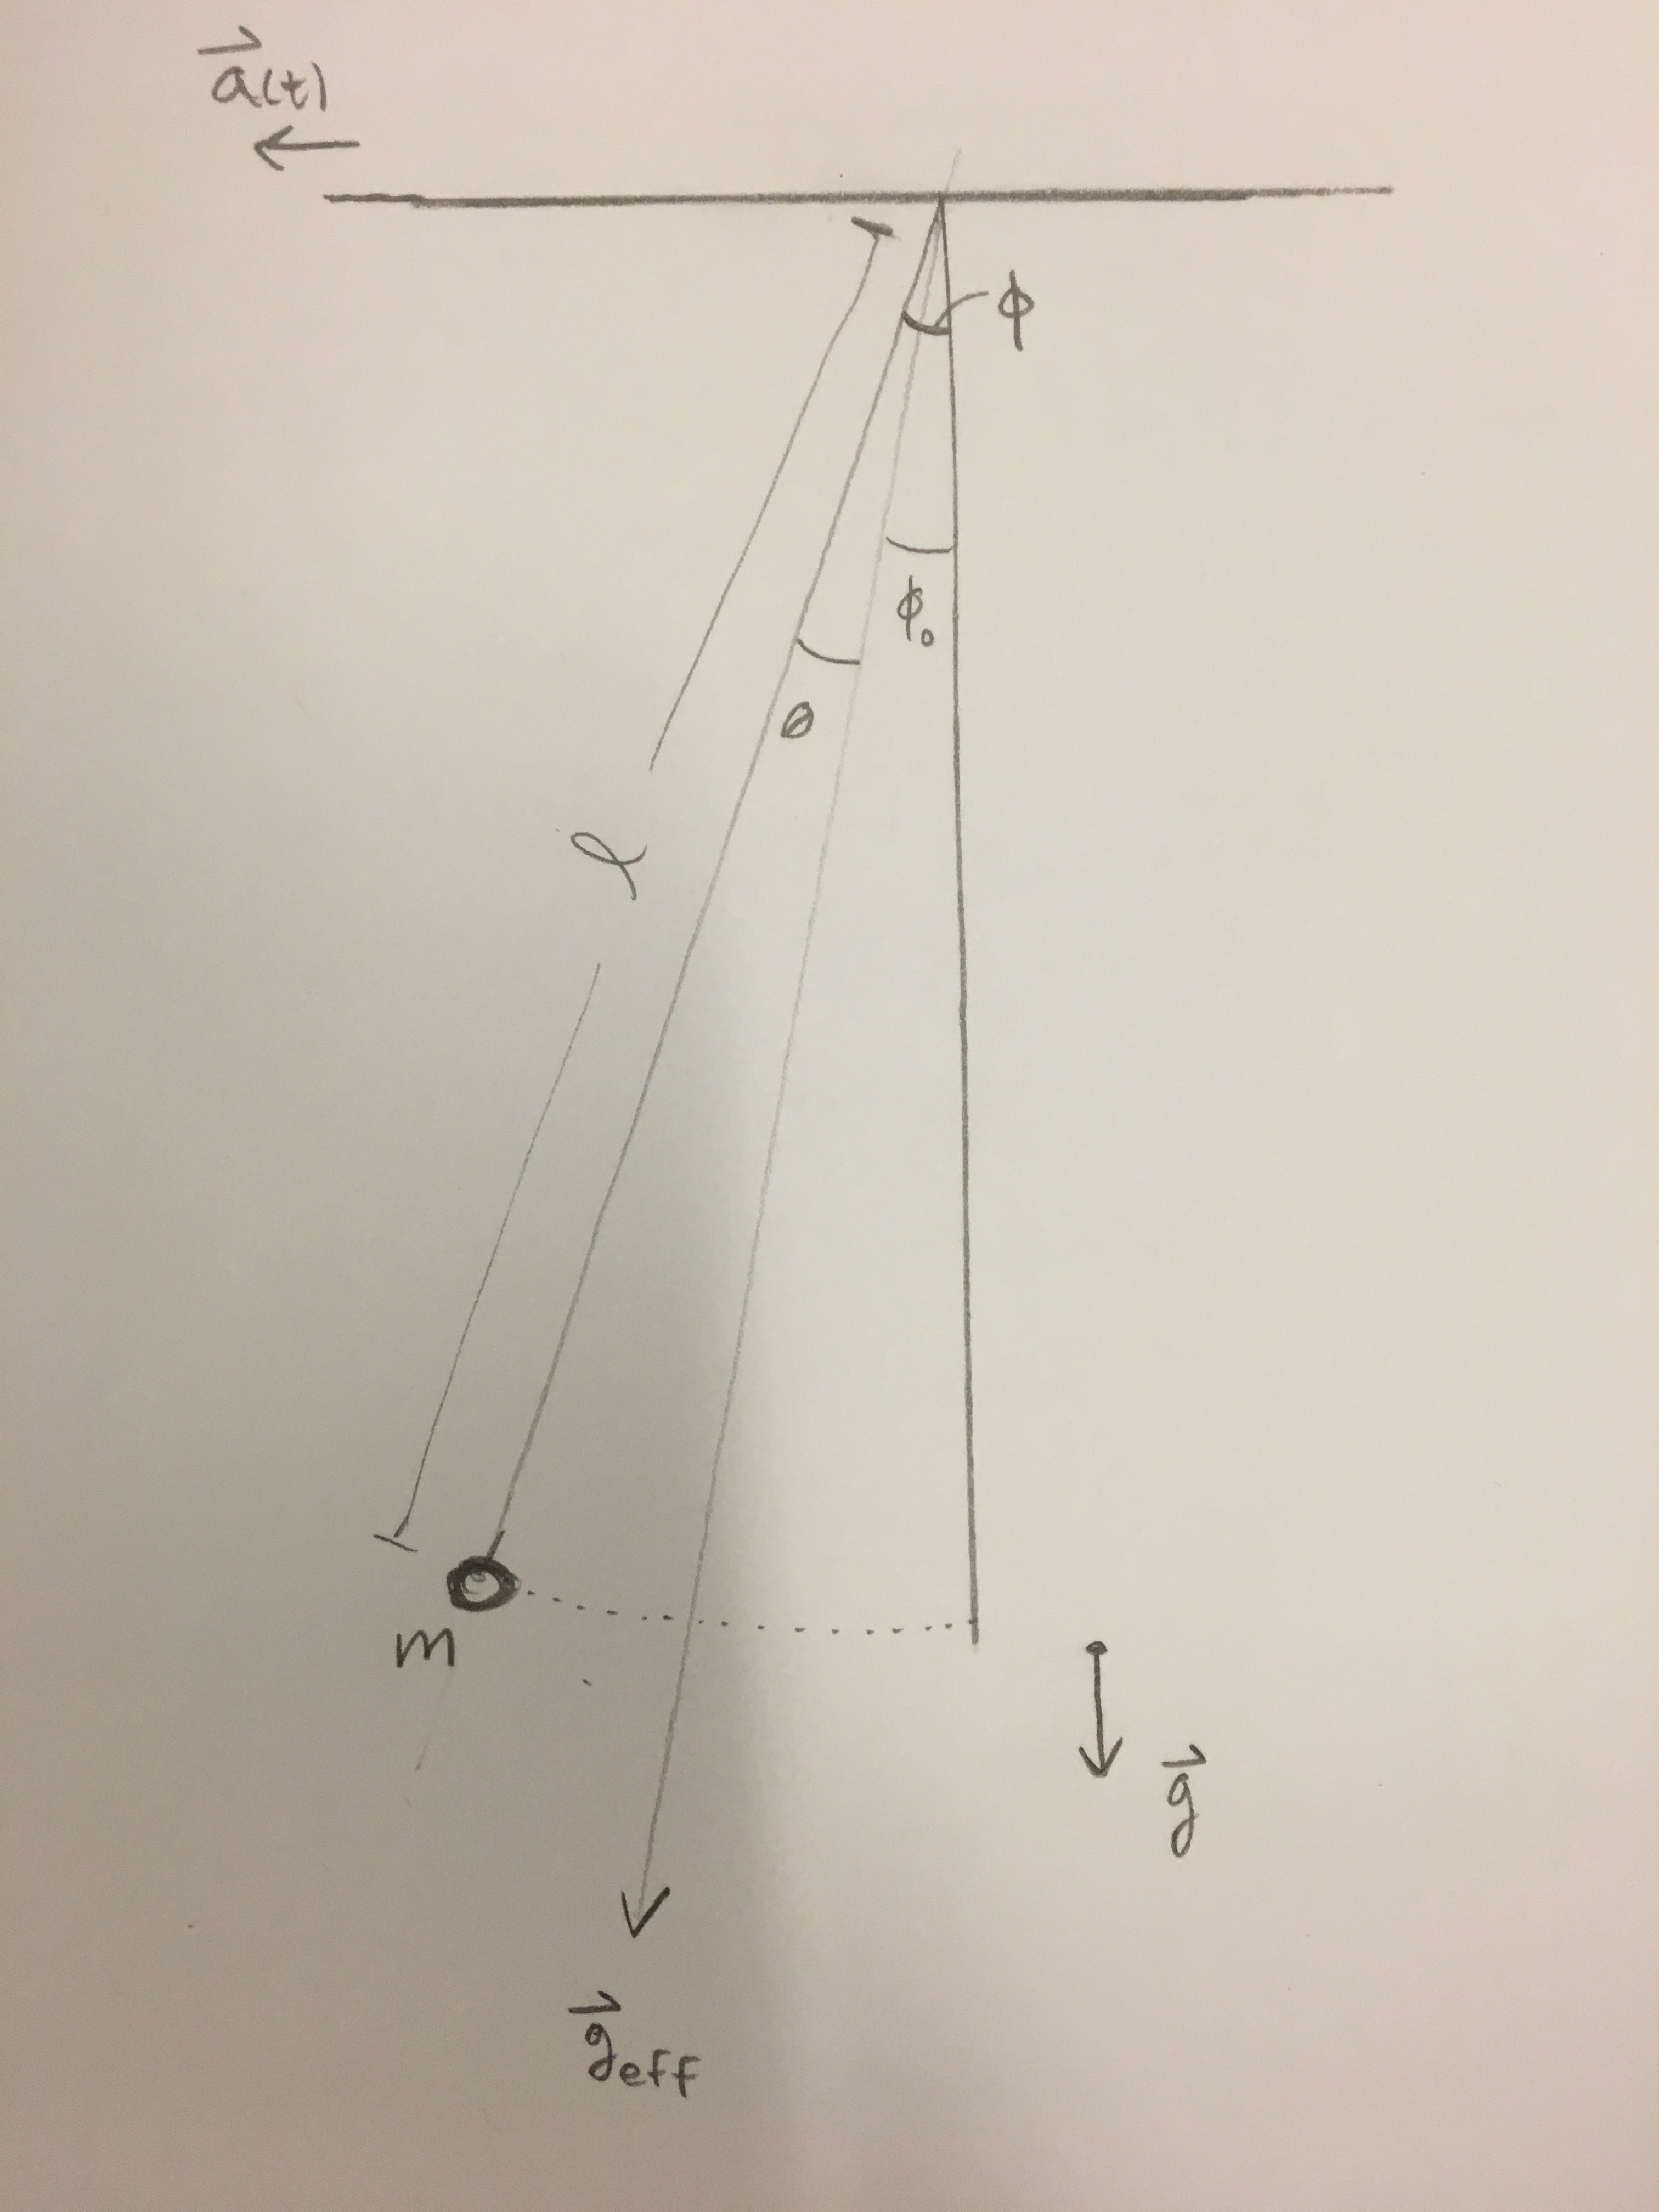
\includegraphics[width=.8\textwidth]{pendulum.jpg}
    \caption{Pendulum that starts at rest in an accelerating frame. If the acceleration is not constant then the apparent vertical, and thus $\phi_0$ will change with time}
\end{figure}

\section{Simulations}

Give a schematic of the experimental setup(s) used in the experiment (see
figure~\ref{fig:samplesetup}). Give the description of  abbreviations
either in the figure caption or in the text. Write a description of what is
going on. 

\subsection{TASK1}

\subsection{TASK2}

\subsection{TASK3}

\subsection{TASK4}

\subsection{TASK5}

%\begin{figure}[ht] 
        % read manual to see what [ht] means and for other possible options
%        \centering \includegraphics[width=0.8\columnwidth]{sr_setup}
        % note that in above figure file name, "sr_setup",
        % the file extension is missing. LaTeX is smart enough to find
        % apropriate one (i.e. pdf, png, etc.)
        % You can add this extention yourself as it seen below
        % both notations are correct but above has more flexibility
        %\includegraphics[width=1.0\columnwidth]{sr_setup.pdf}
%        \caption{
%                \label{fig:samplesetup} % spaces are big no-no withing labels
                % things like fig: are optional in the label but it helps
                % to orient yourself when you have multiple figures,
                % equations and tables
%                Every figure MUST have a caption.
%        }
%\end{figure}

and eventually arrived to the
balanced photodiode as seen in the figure~\ref{fig:samplesetup}.


\section{Results}

In this section you will need to show your experimental results. Use tables and
graphs when it is possible. Table~\ref{tbl:bins} is an example.

\begin{table}[ht]
\begin{center}
\caption{Every table needs a caption.}
\label{tbl:bins} % spaces are big no-no withing labels
\begin{tabular}{|cc|} 
\hline
\multicolumn{1}{|c}{$x$ (m)} & \multicolumn{1}{c|}{$V$ (V)} \\
\hline
0.0044151 &   0.0030871 \\
0.0021633 &   0.0021343 \\
0.0003600 &   0.0018642 \\
0.0023831 &   0.0013287 \\
\hline
\end{tabular}
\end{center}
\end{table}

Analysis of equation~\ref{eq:equation1} shows ...

\blindtext

\begin{figure}
    \centering
    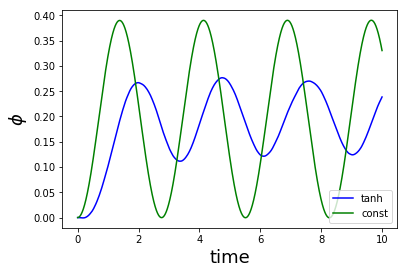
\includegraphics[width=.7\textwidth]{tanh_vs_const_1.png}
    \caption{Hyperbolic tangent acceleration vs immediate constant acceleration. The slow approach to the same asymptotic value of 2 meters per second per second induces a lag in the oscillation and also diminishes the amplitude of oscillation.}
\end{figure}

For example, it is easy to conclude that the
experiment and theory match each other rather well if you look at
Fig.~\ref{fig:samplesetup} and Fig.~\ref{fig:exp_plots}.


\section{Conclusions}
Here you briefly summarize your findings. Did you learn any new physics? Was everything as expected?

\section{Future Work}
Since you had limited time to work on this project, what questions are left outstanding? What would be your next steps? 

%\cite{UMS}

%++++++++++++++++++++++++++++++++++++++++
% References section will be created automatically 
% with inclusion of "thebibliography" environment
% as it shown below. See text starting with line
% \begin{thebibliography}{99}
% Note: with this approach it is YOUR responsibility to put them in order
% of appearance.

\bibliography{project}


\end{document}
